
%% bare_conf.tex
%% V1.3
%% 2007/01/11
%% by Michael Shell
%% See:
%% http://www.michaelshell.org/
%% for current contact information.
%%
%% This is a skeleton file demonstrating the use of IEEEtran.cls
%% (requires IEEEtran.cls version 1.7 or later) with an IEEE conference paper.
%%
%% Support sites:
%% http://www.michaelshell.org/tex/ieeetran/
%% http://www.ctan.org/tex-archive/macros/latex/contrib/IEEEtran/
%% and
%% http://www.ieee.org/

%%*************************************************************************
%% Legal Notice:
%% This code is offered as-is without any warranty either expressed or
%% implied; without even the implied warranty of MERCHANTABILITY or
%% FITNESS FOR A PARTICULAR PURPOSE! 
%% User assumes all risk.
%% In no event shall IEEE or any contributor to this code be liable for
%% any damages or losses, including, but not limited to, incidental,
%% consequential, or any other damages, resulting from the use or misuse
%% of any information contained here.
%%
%% All comments are the opinions of their respective authors and are not
%% necessarily endorsed by the IEEE.
%%
%% This work is distributed under the LaTeX Project Public License (LPPL)
%% ( http://www.latex-project.org/ ) version 1.3, and may be freely used,
%% distributed and modified. A copy of the LPPL, version 1.3, is included
%% in the base LaTeX documentation of all distributions of LaTeX released
%% 2003/12/01 or later.
%% Retain all contribution notices and credits.
%% ** Modified files should be clearly indicated as such, including  **
%% ** renaming them and changing author support contact information. **
%%
%% File list of work: IEEEtran.cls, IEEEtran_HOWTO.pdf, bare_adv.tex,
%%                    bare_conf.tex, bare_jrnl.tex, bare_jrnl_compsoc.tex
%%*************************************************************************

% *** Authors should verify (and, if needed, correct) their LaTeX system  ***
% *** with the testflow diagnostic prior to trusting their LaTeX platform ***
% *** with production work. IEEE's font choices can trigger bugs that do  ***
% *** not appear when using other class files.                            ***
% The testflow support page is at:
% http://www.michaelshell.org/tex/testflow/



% Note that the a4paper option is mainly intended so that authors in
% countries using A4 can easily print to A4 and see how their papers will
% look in print - the typesetting of the document will not typically be
% affected with changes in paper size (but the bottom and side margins will).
% Use the testflow package mentioned above to verify correct handling of
% both paper sizes by the user's LaTeX system.
%
% Also note that the "draftcls" or "draftclsnofoot", not "draft", option
% should be used if it is desired that the figures are to be displayed in
% draft mode.
%
\documentclass[conference]{IEEEtran}
\usepackage{blindtext, graphicx}
\usepackage{multirow}
\usepackage{caption}
% Add the compsoc option for Computer Society conferences.
%
% If IEEEtran.cls has not been installed into the LaTeX system files,
% manually specify the path to it like:
% \documentclass[conference]{../sty/IEEEtran}





% Some very useful LaTeX packages include:
% (uncomment the ones you want to load)


% *** MISC UTILITY PACKAGES ***
%
%\usepackage{ifpdf}
% Heiko Oberdiek's ifpdf.sty is very useful if you need conditional
% compilation based on whether the output is pdf or dvi.
% usage:
% \ifpdf
%   % pdf code
% \else
%   % dvi code
% \fi
% The latest version of ifpdf.sty can be obtained from:
% http://www.ctan.org/tex-archive/macros/latex/contrib/oberdiek/
% Also, note that IEEEtran.cls V1.7 and later provides a builtin
% \ifCLASSINFOpdf conditional that works the same way.
% When switching from latex to pdflatex and vice-versa, the compiler may
% have to be run twice to clear warning/error messages.






% *** CITATION PACKAGES ***
%
%\usepackage{cite}
% cite.sty was written by Donald Arseneau
% V1.6 and later of IEEEtran pre-defines the format of the cite.sty package
% \cite{} output to follow that of IEEE. Loading the cite package will
% result in citation numbers being automatically sorted and properly
% "compressed/ranged". e.g., [1], [9], [2], [7], [5], [6] without using
% cite.sty will become [1], [2], [5]--[7], [9] using cite.sty. cite.sty's
% \cite will automatically add leading space, if needed. Use cite.sty's
% noadjust option (cite.sty V3.8 and later) if you want to turn this off.
% cite.sty is already installed on most LaTeX systems. Be sure and use
% version 4.0 (2003-05-27) and later if using hyperref.sty. cite.sty does
% not currently provide for hyperlinked citations.
% The latest version can be obtained at:
% http://www.ctan.org/tex-archive/macros/latex/contrib/cite/
% The documentation is contained in the cite.sty file itself.






% *** GRAPHICS RELATED PACKAGES ***
%
\ifCLASSINFOpdf
  % \usepackage[pdftex]{graphicx}
  % declare the path(s) where your graphic files are
  % \graphicspath{{../pdf/}{../jpeg/}}
  % and their extensions so you won't have to specify these with
  % every instance of \includegraphics
  % \DeclareGraphicsExtensions{.pdf,.jpeg,.png}
\else
  % or other class option (dvipsone, dvipdf, if not using dvips). graphicx
  % will default to the driver specified in the system graphics.cfg if no
  % driver is specified.
  % \usepackage[dvips]{graphicx}
  % declare the path(s) where your graphic files are
  % \graphicspath{{../eps/}}
  % and their extensions so you won't have to specify these with
  % every instance of \includegraphics
  % \DeclareGraphicsExtensions{.eps}
\fi
% graphicx was written by David Carlisle and Sebastian Rahtz. It is
% required if you want graphics, photos, etc. graphicx.sty is already
% installed on most LaTeX systems. The latest version and documentation can
% be obtained at: 
% http://www.ctan.org/tex-archive/macros/latex/required/graphics/
% Another good source of documentation is "Using Imported Graphics in
% LaTeX2e" by Keith Reckdahl which can be found as epslatex.ps or
% epslatex.pdf at: http://www.ctan.org/tex-archive/info/
%
% latex, and pdflatex in dvi mode, support graphics in encapsulated
% postscript (.eps) format. pdflatex in pdf mode supports graphics
% in .pdf, .jpeg, .png and .mps (metapost) formats. Users should ensure
% that all non-photo figures use a vector format (.eps, .pdf, .mps) and
% not a bitmapped formats (.jpeg, .png). IEEE frowns on bitmapped formats
% which can result in "jaggedy"/blurry rendering of lines and letters as
% well as large increases in file sizes.
%
% You can find documentation about the pdfTeX application at:
% http://www.tug.org/applications/pdftex





% *** MATH PACKAGES ***
%
%\usepackage[cmex10]{amsmath}
% A popular package from the American Mathematical Society that provides
% many useful and powerful commands for dealing with mathematics. If using
% it, be sure to load this package with the cmex10 option to ensure that
% only type 1 fonts will utilized at all point sizes. Without this option,
% it is possible that some math symbols, particularly those within
% footnotes, will be rendered in bitmap form which will result in a
% document that can not be IEEE Xplore compliant!
%
% Also, note that the amsmath package sets \interdisplaylinepenalty to 10000
% thus preventing page breaks from occurring within multiline equations. Use:
%\interdisplaylinepenalty=2500
% after loading amsmath to restore such page breaks as IEEEtran.cls normally
% does. amsmath.sty is already installed on most LaTeX systems. The latest
% version and documentation can be obtained at:
% http://www.ctan.org/tex-archive/macros/latex/required/amslatex/math/





% *** SPECIALIZED LIST PACKAGES ***
%
%\usepackage{algorithmic}
% algorithmic.sty was written by Peter Williams and Rogerio Brito.
% This package provides an algorithmic environment fo describing algorithms.
% You can use the algorithmic environment in-text or within a figure
% environment to provide for a floating algorithm. Do NOT use the algorithm
% floating environment provided by algorithm.sty (by the same authors) or
% algorithm2e.sty (by Christophe Fiorio) as IEEE does not use dedicated
% algorithm float types and packages that provide these will not provide
% correct IEEE style captions. The latest version and documentation of
% algorithmic.sty can be obtained at:
% http://www.ctan.org/tex-archive/macros/latex/contrib/algorithms/
% There is also a support site at:
% http://algorithms.berlios.de/index.html
% Also of interest may be the (relatively newer and more customizable)
% algorithmicx.sty package by Szasz Janos:
% http://www.ctan.org/tex-archive/macros/latex/contrib/algorithmicx/




% *** ALIGNMENT PACKAGES ***
%
%\usepackage{array}
% Frank Mittelbach's and David Carlisle's array.sty patches and improves
% the standard LaTeX2e array and tabular environments to provide better
% appearance and additional user controls. As the default LaTeX2e table
% generation code is lacking to the point of almost being broken with
% respect to the quality of the end results, all users are strongly
% advised to use an enhanced (at the very least that provided by array.sty)
% set of table tools. array.sty is already installed on most systems. The
% latest version and documentation can be obtained at:
% http://www.ctan.org/tex-archive/macros/latex/required/tools/


%\usepackage{mdwmath}
%\usepackage{mdwtab}
% Also highly recommended is Mark Wooding's extremely powerful MDW tools,
% especially mdwmath.sty and mdwtab.sty which are used to format equations
% and tables, respectively. The MDWtools set is already installed on most
% LaTeX systems. The lastest version and documentation is available at:
% http://www.ctan.org/tex-archive/macros/latex/contrib/mdwtools/


% IEEEtran contains the IEEEeqnarray family of commands that can be used to
% generate multiline equations as well as matrices, tables, etc., of high
% quality.


%\usepackage{eqparbox}
% Also of notable interest is Scott Pakin's eqparbox package for creating
% (automatically sized) equal width boxes - aka "natural width parboxes".
% Available at:
% http://www.ctan.org/tex-archive/macros/latex/contrib/eqparbox/





% *** SUBFIGURE PACKAGES ***
%\usepackage[tight,footnotesize]{subfigure}
% subfigure.sty was written by Steven Douglas Cochran. This package makes it
% easy to put subfigures in your figures. e.g., "Figure 1a and 1b". For IEEE
% work, it is a good idea to load it with the tight package option to reduce
% the amount of white space around the subfigures. subfigure.sty is already
% installed on most LaTeX systems. The latest version and documentation can
% be obtained at:
% http://www.ctan.org/tex-archive/obsolete/macros/latex/contrib/subfigure/
% subfigure.sty has been superceeded by subfig.sty.



%\usepackage[caption=false]{caption}
%\usepackage[font=footnotesize]{subfig}
% subfig.sty, also written by Steven Douglas Cochran, is the modern
% replacement for subfigure.sty. However, subfig.sty requires and
% automatically loads Axel Sommerfeldt's caption.sty which will override
% IEEEtran.cls handling of captions and this will result in nonIEEE style
% figure/table captions. To prevent this problem, be sure and preload
% caption.sty with its "caption=false" package option. This is will preserve
% IEEEtran.cls handing of captions. Version 1.3 (2005/06/28) and later 
% (recommended due to many improvements over 1.2) of subfig.sty supports
% the caption=false option directly:
%\usepackage[caption=false,font=footnotesize]{subfig}
%
% The latest version and documentation can be obtained at:
% http://www.ctan.org/tex-archive/macros/latex/contrib/subfig/
% The latest version and documentation of caption.sty can be obtained at:
% http://www.ctan.org/tex-archive/macros/latex/contrib/caption/




% *** FLOAT PACKAGES ***
%
%\usepackage{fixltx2e}
% fixltx2e, the successor to the earlier fix2col.sty, was written by
% Frank Mittelbach and David Carlisle. This package corrects a few problems
% in the LaTeX2e kernel, the most notable of which is that in current
% LaTeX2e releases, the ordering of single and double column floats is not
% guaranteed to be preserved. Thus, an unpatched LaTeX2e can allow a
% single column figure to be placed prior to an earlier double column
% figure. The latest version and documentation can be found at:
% http://www.ctan.org/tex-archive/macros/latex/base/



%\usepackage{stfloats}
% stfloats.sty was written by Sigitas Tolusis. This package gives LaTeX2e
% the ability to do double column floats at the bottom of the page as well
% as the top. (e.g., "\begin{figure*}[!b]" is not normally possible in
% LaTeX2e). It also provides a command:
%\fnbelowfloat
% to enable the placement of footnotes below bottom floats (the standard
% LaTeX2e kernel puts them above bottom floats). This is an invasive package
% which rewrites many portions of the LaTeX2e float routines. It may not work
% with other packages that modify the LaTeX2e float routines. The latest
% version and documentation can be obtained at:
% http://www.ctan.org/tex-archive/macros/latex/contrib/sttools/
% Documentation is contained in the stfloats.sty comments as well as in the
% presfull.pdf file. Do not use the stfloats baselinefloat ability as IEEE
% does not allow \baselineskip to stretch. Authors submitting work to the
% IEEE should note that IEEE rarely uses double column equations and
% that authors should try to avoid such use. Do not be tempted to use the
% cuted.sty or midfloat.sty packages (also by Sigitas Tolusis) as IEEE does
% not format its papers in such ways.





% *** PDF, URL AND HYPERLINK PACKAGES ***
%
%\usepackage{url}
% url.sty was written by Donald Arseneau. It provides better support for
% handling and breaking URLs. url.sty is already installed on most LaTeX
% systems. The latest version can be obtained at:
% http://www.ctan.org/tex-archive/macros/latex/contrib/misc/
% Read the url.sty source comments for usage information. Basically,
% \url{my_url_here}.





% *** Do not adjust lengths that control margins, column widths, etc. ***
% *** Do not use packages that alter fonts (such as pslatex).         ***
% There should be no need to do such things with IEEEtran.cls V1.6 and later.
% (Unless specifically asked to do so by the journal or conference you plan
% to submit to, of course. )


% correct bad hyphenation here
\hyphenation{op-tical net-works semi-conduc-tor}


\begin{document}
%
% paper title
% can use linebreaks \\ within to get better formatting as desired
\title{Key2Vec: Automatic Ranked Keyword Extraction from Scientific Articles using Keyphrase Embeddings}


% author names and affiliations
% use a multiple column layout for up to three different
% affiliations
\author{\IEEEauthorblockN{Anonymous}
\IEEEauthorblockA{Anonymous}
\and
\IEEEauthorblockN{Anonymous}
\IEEEauthorblockA{Anonymous}
}

% conference papers do not typically use \thanks and this command
% is locked out in conference mode. If really needed, such as for
% the acknowledgment of grants, issue a \IEEEoverridecommandlockouts
% after \documentclass

% for over three affiliations, or if they all won't fit within the width
% of the page, use this alternative format:
% 
%\author{\IEEEauthorblockN{Michael Shell\IEEEauthorrefmark{1},
%Homer Simpson\IEEEauthorrefmark{2},
%James Kirk\IEEEauthorrefmark{3}, 
%Montgomery Scott\IEEEauthorrefmark{3} and
%Eldon Tyrell\IEEEauthorrefmark{4}}
%\IEEEauthorblockA{\IEEEauthorrefmark{1}School of Electrical and Computer Engineering\\
%Georgia Institute of Technology,
%Atlanta, Georgia 30332--0250\\ Email: see http://www.michaelshell.org/contact.html}
%\IEEEauthorblockA{\IEEEauthorrefmark{2}Twentieth Century Fox, Springfield, USA\\
%Email: homer@thesimpsons.com}
%\IEEEauthorblockA{\IEEEauthorrefmark{3}Starfleet Academy, San Francisco, California 96678-2391\\
%Telephone: (800) 555--1212, Fax: (888) 555--1212}
%\IEEEauthorblockA{\IEEEauthorrefmark{4}Tyrell Inc., 123 Replicant Street, Los Angeles, California 90210--4321}}




% use for special paper notices
%\IEEEspecialpapernotice{(Invited Paper)}




% make the title area
\maketitle

%Keywords can be used in processes such as indexing, clustering, classification, summarization, auto-tagging, and many other tasks responsible for organizing information.
\begin{abstract}
%\boldmath
Keyword extraction is a fundamental task in natural language processing that facilitates mapping of documents to a concise set of representative single and multi-word phrases. Keywords from text documents are primarily extracted using supervised and unsupervised approaches. In this paper, we present a novel and effective unsupervised technique named \textit{Key2Vec} that extensively takes into account neural keyphrase embeddings for extracting and ranking keywords from scientific articles. We introduce an efficient way of processing text documents and training keyphrase embeddings for the purpose of extracting and ranking keywords. We share a new evaluation dataset used for choosing the underlying model for \textit{Key2Vec}, which is based on semantic similarity of textual segments.  The evaluations for ranked keyword extraction are performed on two benchmark datasets comprising of short abstracts (Inspec), and long scientific papers (SemEval 2010), and is shown to produce results better than the state-of-the-art systems. We also show how keyphrase embeddings could be further used for capturing semantic similarity between text documents, and for performing efficient extractive summarization using the \textit{Key2Vec} framework.
%\blindtext[1]
\end{abstract}
% IEEEtran.cls defaults to using nonbold math in the Abstract.
% This preserves the distinction between vectors and scalars. However,
% if the journal you are submitting to favors bold math in the abstract,
% then you can use LaTeX's standard command \boldmath at the very start
% of the abstract to achieve this. Many IEEE journals frown on math
% in the abstract anyway.

% Note that keywords are not normally used for peerreview papers.
\begin{IEEEkeywords}
keyword extraction, keyword assignment, ranked keyword extraction, information extraction, phrase embedding, keyphrase embedding, neural language model.
\end{IEEEkeywords}






% For peer review papers, you can put extra information on the cover
% page as needed:
% \ifCLASSOPTIONpeerreview
% \begin{center} \bfseries EDICS Category: 3-BBND \end{center}
% \fi
%
% For peerreview papers, this IEEEtran command inserts a page break and
% creates the second title. It will be ignored for other modes.
\IEEEpeerreviewmaketitle


\section{Introduction}
Keywords are single or multi-word linguistic units that represent the salient aspects of a document. In this paper, we use the term
keyword uniformly to represent both single and multi-word phrases. Keywords are useful in many tasks
such as indexing documents \cite{gutwin1999improving}, summarization \cite{litvak2008graph}, clustering \cite{hammouda2005corephrase}, ontology creation \cite{gulla2007ontology}, classification \cite{hulth2006study}, auto-tagging \cite{wu2010automatic} and visualization of text \cite{collins2009parallel}. Due to its widespread use, keyword extraction has received a lot of attention from researchers.

In order to push the state-of-the-art performances of keyword extraction systems, the research community has been hosting shared tasks like SemeEval 2010 Task 5 \cite{kim2010semeval} and SemEval 2017 Task 10 \cite{augenstein2017semeval}. However, the task is far from solved and the performances of the present systems are worse in comparison to many other NLP tasks \cite{liu2010automatic}. Some of the major challenges are the varied length of the documents to be processed, their structural inconsistency and developing strategies that can perform well in different domains \cite{hasan2014automatic}.

The task of ranked keyword extraction from scientific articles and identifying relationships between them is of great interest to scientific publishers as it helps to recommend articles to readers, highlight
missing citations to authors, identify potential reviewers for submissions, and analyse research trends over time \cite{augenstein2017semeval}. Although scientific articles usually provide them, most of the documents have no associated keywords. Therefore, the problem of automatically extracting the most representative keywords from scientific articles is an active field of research. 

Methods for automatic keyword extraction are mainly divided into two categories: \textit{supervised} and \textit{unsupervised}. 
Supervised methods approach the problem of keyword extraction as a binary classification problem \cite{hasan2014automatic}, whereas the unsupervised methods are mostly based on TFIDF, clustering, and graph-based ranking \cite{hasan2010conundrums}. On presence of domain-specific data, supervised methods have shown better performance than the unsupervised methods. The unsupervised methods have the advantage of not requiring any training data and can produce results in any domain. However, the assumptions of unsupervised methods do not hold for every type of document. 

With recent advancements in deep learning techniques applied to natural language processing, the latest trend is to represent words as dense real-valued vectors obtained by training a shallow neural network on a fixed vocabulary. These distributional representation of words are popularly known as word embeddings. These neural representations have been shown to equal or outperform other methods (e.g. LSA, SVD) \cite{baroni2014don}. The vector representation of words, are supposed to preserve the semantic and syntactic similarities between them. They have been shown to be useful for several natural language processing (NLP) tasks, like part-of-speech tagging, chunking, named entity recognition, semantic role labeling, syntactic parsing, and also for speech processing \cite{collobert2011natural}. Some of the most popular approaches for generating word embeddings are Word2Vec \cite{mikolov2013distributed}, Glove \cite{pennington2014glove} and Fasttext \cite{bojanowski2016enriching}.

%These procedures for generating word and text embeddings have been popularized in the form of toolkits that are easy to use with various programming languages and can be trained on huge corpus using distributed processing environments. The main benefit of these embedding methods is that they can be trained in an unsupervised way, without any need for expensive annotation and are derived from large unannotated corpora.  The trained models can then be deployed in a variety of applications. In this paper, we have used Word2Vec, Fasttext and Doc2Vec approaches for generating word and document embeddings for the purpose of content based recommendations. We give a brief overview of each of them.
%
%
%In this paper we introduce a new approach that knits together techniques from supervised and unsupervised paradigms in the form of a robust framework, which leverages distributed representation of keywords in order to produce state-of-the-art results in keyword extraction from text documents. Due to extensive use of keyword embeddings trained using Word2Vec \cite{mikolov2013distributed} and its effectiveness, we name our framework as \textit{Key2Vec}. Table ~\ref{sample-result}, shows sample keywords automatically extracted by \textit{Key2Vec} from a research article abstract in the Inspec corpus. The main contributions of our work towards ranked keyword extraction are:
%\begin{itemize}
%  \item Effective application of distributed representation of keywords in the form of \textit{keyword embeddings}.
%  \item Introduction of new \textit{heuristics for identification of candidate keywords} by leveraging \textit{keyword embeddings}.
%  \item \textit{Use of keyword embeddings for generating features useful for supervised scoring} and \textit{unsupervised ranking} of candidate keywords.
%  \item \textit{Hybrid approach} taking advantages of supervised and unsupervised techniques for developing a robust methodology.
%  \item A \textit{generic framework} (\textit{Key2Vec}) for extracting and ranking keywords from text documents related to any domain.
%\end{itemize}


In this paper, we introduce the notion of \textit{keyphrase embeddings}, and show how they could be trained in a simple and effective way using already existing algorithms belonging to the neural word embedding family (Word2Vec and Fasttext). Instead of distributional representation of words we produce distributional representation of keyphrases for the purpose of ranked keyword extraction from scientific articles. We call our methodology as \textit{Key2Vec}. We also propose a text processing pipeline for training keyphrase embeddings, which enables intelligent tokenization of text into a mix of unigram and meaningful chunks of multi-gram tokens. We show how the embedding models trained using our strategy, can be advantageously used for representing keyphrases and text snippets as dense vectors that are further used for calculating semantic and syntactic similarities. We fully rely on training high quality embedding models and effectively use the similarities between the distributional representation of keyphrases for ranking representative keywords from scientific documents. Table \ref{sample-result}, shows keywords extracted from a sample research article abstract, by using \textit{Key2Vec}.  

\begin{table}[htbp]
\footnotesize
\centering
\caption{\small Keywords extracted by using \textit{Key2Vec} from a sample research article abstract.}
\tabcolsep=0.10cm
\scalebox{1.0}{
\begin{tabular}{l}
\begin{tabular}[c]{@{}l@{}}\textbf{Title:} Identification of states of complex systems with estimation of \\ admissible measurement errors on the basis of fuzzy information.\\ \textbf{Abstract:} The problem of identification of states of complex systems on the \\ basis of fuzzy values of informative attributes is considered. Some estimates \\ of a maximally admissible degree of measurement error are obtained that \\ make it possible, using the apparatus of fuzzy set theory, to correctly identify \\ the current state of a system.\\  \textbf{Automatically identified keywords:} \textit{complex systems, fuzzy information,} \\ \textit{admissible measurement errors, fuzzy values, informative attributes} \\ \textit{measurement error, maximally admissible degree, fuzzy set theory}\\ \textbf{Manually assigned keywords:} \textit{complex system state identification,} \\ \textit{admissible measurement errors, informative attributes, measurement errors} \\ \textit{fuzzy set theory}\end{tabular}
\end{tabular}}
\label{sample-result}
\end{table}


For the purpose of evaluating our embedding models on different similarity tasks, we develop a new evaluation dataset\footnote{www.example.com} (Section \ref{embedding-model-selection}), from an exisiting dataset \cite{dai2015document}. We share the dataset with the community believing that it would facilitate training of better keyphrase embedding models useful for ranked keyword extraction. Contrary, to the analogy task that is widely used for intrinsic evaluation of word embeddings, this dataset can be used for evaluating phrase and word embeddings on similarity tasks, whenever they are being trained for a downstream process that has semantic and syntactic similarity between distributional representation of text at its core. We perform such an evaluation and show that our keyphrase embeddings are more effective in capturing semantic similarity between text documents at lower dimensions, than normal word embeddings, when trained using the same parameters (Section \ref{discussion}).

%\textit{Given a text document $D_{i}$, and a set of candidate phrases $C_{i} = \{ c_{1},c_{2},...c_{n}\}$, extracted from $D_{i}$, the task is to find a ranked set of keywords $K_{i} = \{ k_{1},k_{2},...k_{k}\}$, $K_{i}\subseteq C_{i}$, such that $K_{i}$ contains the candidate phrases from $C_{i}$, that represents the main topics covered in the document $D_{i}$.}

We not only aim at extracting the keywords that are statistically relevant for the given document, as mostly attempted by previous studies \cite{hasan2014automatic}, but also to rightly identify meaningful keyphrases that are most semantically related to the main theme of the document. We are motivated by the following properties for the top-K keywords that we select using \textit{Key2Vec} as mentioned in \cite{liu2009clustering}.

\begin{itemize}
\item \textit{Understandability} - The ranked keywords should be understandable to readers, which is made possible by chosing grammatically correct and meaningful phrases that possess the characteristic of high readability by humans. For example, the phrase \textit{scientific articles} has more understandability than the individual words \textit{scientific} and \textit{articles}.  
\item \textit{Relevancy} - The top-K keywords should be semantically related to the central theme of the document.
\item \textit{Good Coverage} - The keywords should cover all the major topics discussed in the document.
\end{itemize}

This intrigued us to look at the route of training keyphrase embeddings as presented in this paper, rather than first training embedding models for unigram words and then combining their dense vector representations to obtain similar representations for multi-word phrases. Training keyphrase embeddings for extracting and ranking keywords is relatively a new problem and has not been thoroughly explored. Researchers have just started exploring the advantages of neural word embeddings for representing semantic similarities between words that are further leveraged in graph-based ranking algorithms, in order to rank extracted keywords \cite{wang2015using}. To our knowledge, keyphrase embeddings have not been used for ranked keyword extraction and summarization, and this work is the first attempt to do so. 


Some of the major contributions of this paper are,
\begin{itemize}
  \item \textit{Intelligent processing of text for training neural keyphrase embeddings}.
  \item Effective \textit{application of keyphrase embeddings for extraction and ranking of keywords}, producing state-of-the-art results.
  %\item Introduction of new \textit{heuristics for identification of candidate keywords} by leveraging \textit{phrase embeddings}.
  \item \textit{A dataset for evaluating the quality of embedding models}, trained for the purpose of capturing semantic similarities between different types of textual units.
  \item A new \textit{generic framework} (\textit{Key2Vec}), based on distributional semantics, for \textit{ranked keyword extraction}, and \textit{summarization}.
\end{itemize}

The rest of the paper is organized as follows. In Section \ref{related_work}, we discuss about the background literature and works relevant to ours. We fully describe our methodology in Section \ref{methodology}, and present our empirical experiment results in Section \ref{experiments}. We discuss our learnings and applications of our framework in Section \ref{discussion}, followed by our conclusion and plans for future work in Section \ref{conclusion}

\section{Related Work\label{related_work}}

In this section, we give a brief overview of the previous works that are most relevant to this paper. As we use different word embedding techniques in order to train phrase embeddings, we first present a brief review of the popular neural word and phrase embedding approaches (Section \ref{word-embedding} and Section \ref{phrase-embedding}, respectively). Present keyword extraction systems primarily operate by using some heuristics for choosing candidate keywords (Section \ref{cand-select}) that are further ranked by using supervised (Section \ref{supervised-review}) or unsupervised (Section \ref{unsupervised-review}) approaches. We point out some of the strategies and whenever necessary, explain where we differ.

\subsection{Neural Word and Phrase Embeddings\label{word-embedding}}
One of the dominant trends in Natural Language Processing (NLP) at the moment is the use of word embeddings trained using shallow neural networks. also known as neural word embeddings. These word embeddings are distributional representations of words, whose relative similarities correlate with semantic similarities. The real-valued vector representation of words trained using neural networks have been widely used as representational basis for many downstream tasks like text classification \cite{joulin2016bag}, document clustering, part of speech tagging, named entity recognition, sentiment analysis, recommendations, etc.

The term word embedding was originally coined by Bengio et al. \cite{bengio2003neural}, in 2003. Initially, word embeddings were just a by-product of training neural language models. It was only in 2008, that Collobert and Weston \cite{collobert2008unified}, showed the effectiveness of using pre-trained word embeddings in various downstream tasks related to natural language processing. But it was after a series of works published by Mikolov et al, \cite{mikolov2013efficient, mikolov2013distributed, le2014distributed} along with the availability of \textit{Word2Vec} tool, that word embeddings became mainstream and gained wide popularity. 

\subsubsection{Candidate Identification Approaches for Ranked Keyword Extraction\label{cand-select}}
One of the first steps in any keyword extraction method is to identify a set of candidate phrases or words in an optimal way, which are further ranked for getting the top representative keywords for a text document. Typical heuristics include different ways of processing the text, like allowing phrases and words with certain parts-of-speech tag combinations \cite{mihalcea2004textrank}, and allowing n-grams \cite{danesh2015sgrank} that satisfy certain statistical criteria. External corpora have also been used for filtering out unimportant phrases and n-grams.

Researchers have devised a plethora of methods for distinguishing between good and bad (or better and worse) keyphrase candidates. The simplest rely solely on frequency statistics, such as TF*IDF or BM25, to score candidates, assuming that a document’s keyphrases tend to be relatively frequent within the document as compared to an external reference corpus. Unfortunately, their performance is mediocre; researchers have demonstrated that the best keyphrases aren’t necessarily the most frequent within a document. (For a statistical analysis of human-generated keyphrases, check out Descriptive Keyphrases for Text Visualization.) A next attempt might score candidates using multiple statistical features combined in an ad hoc or heuristic manner, but this approach only goes so far. More sophisticated methods apply machine learning to the problem. They fall into two broad categories.

\subsubsection{Supervised Approaches for Ranked Keyword Extraction\label{supervised-review}}
Supervised machine learning methods use training data to infer a function that maps a set of input variables called features to some desired (and known) output value; ideally, this function can correctly predict the (unknown) output values of new examples based on their features alone. The two primary developments in supervised approaches to automatic keyphrase extraction deal with task reformulation and feature design.

Early implementations recast the problem of extracting keyphrases from a document as a binary classification problem, in which some fraction of candidates are classified as keyphrases and the rest as non-keyphrases. This is a well-understood problem, and there are many methods to solve it: Naive Bayes, decision trees, and support vector machines, among others. However, this reformulation of the task is conceptually problematic; humans don’t judge keyphrases independently of one another, instead they judge certain phrases as more key than others in a intrinsically relative sense. As such, more recently the problem has been reformulated as a ranking problem, in which a function is trained to rank candidates pairwise according to degree of “keyness”. The best candidates rise to the top, and the top N are taken to be the document’s keyphrases.

The second line of research into supervised approaches has explored a wide variety of features used to discriminate between keyphrases and non-keyphrases. The most common are the aforementioned frequency statistics, along with a grab-bag of other statistical features: phrase length (number of constituent words), phrase position (normalized position within a document of first and/or last occurrence therein), and “supervised keyphraseness” (number of times a keyphrase appears as such in the training data). Some models take advantage of a document’s structural features — titles, abstracts, intros and conclusions, metadata, and so on — because a candidate is more likely to be a keyphrase if it appears in notable sections. Others are external resource-based features: “Wikipedia-based keyphraseness” assumes that keyphrases are more likely to appear as Wiki article links and/or titles, while phrase commonness compares a candidate’s frequency in a document with respect to its frequency in an external corpus. The list of possible features goes on and on.

A well-known implementation of the binary classification method, KEA (as published in Practical Automatic Keyphrase Extraction), used TF*IDF and position of first occurrence (while filtering on phrase length) to identify keyphrases. In A Ranking Approach to Keyphrase Extraction, researchers used a Linear Ranking SVM to rank candidate keyphrases with much success (but failed to give their algorithm a catchy name).

Supervised approaches have generally achieved better performance than unsupervised approaches; however, good training data is hard to find (although here’s a decent place to start), and the danger of training a model that doesn’t generalize to unseen examples is something to always guard against (e.g. through cross-validation).

\subsubsection{Unsupervised Approaches for Ranked Keyword Extraction\label{unsupervised-review}}
Unsupervised machine learning methods attempt to discover the underlying structure of a dataset without the assistance of already-labeled examples (“training data”). The canonical unsupervised approach to automatic keyphrase extraction uses a graph-based ranking method, in which the importance of a candidate is determined by its relatedness to other candidates, where “relatedness” may be measured by two terms’ frequency of co-occurrence or semantic relatedness. This method assumes that more important candidates are related to a greater number of other candidates, and that more of those related candidates are also considered important; it does not, however, ensure that selected keyphrases cover all major topics, although multiple variations try to compensate for this weakness.

Essentially, a document is represented as a network whose nodes are candidate keyphrases (typically only key words) and whose edges (optionally weighted by the degree of relatedness) connect related candidates. Then, a graph-based ranking algorithm, such as Google’s famous PageRank, is run over the network, and the highest-scoring terms are taken to be the document’s keyphrases.

The most famous instantiation of this approach is TextRank; a variation that attempts to ensure good topic coverage is DivRank. For a more extensive breakdown, see Conundrums in Unsupervised Keyphrase Extraction, which includes an example of a topic-based clustering method, the other main class of unsupervised keyphrase extraction algorithms (which I’m not going to delve into).

Unsupervised approaches have at least one notable strength: No training data required! In an age of massive but unlabled datasets, this can be a huge advantage over other approaches. As for disadvantages, unsupervised methods make assumptions that don’t necessarily hold across different domains, and up until recently, their performance has been inferior to supervised methods. Which brings me to the next section.

%\subsection{Problem Statement}


\section{Methodology \label{methodology}}

\subsection{Text Processing \label{text-processing}}

\begin{figure}
\centering
  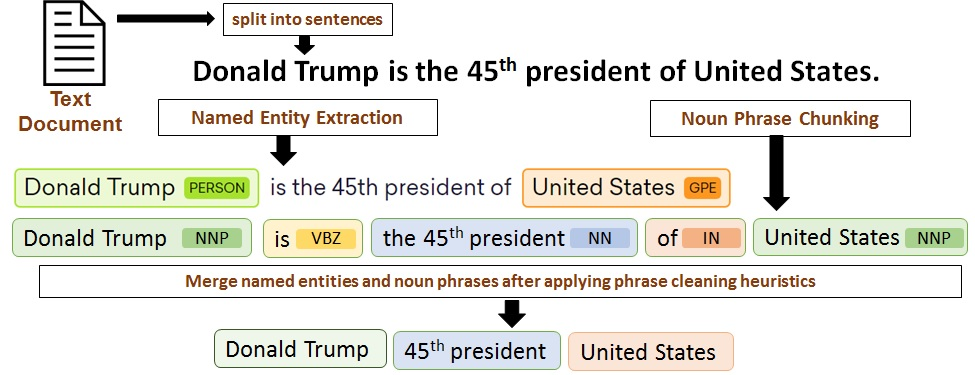
\includegraphics[width=9cm, height=4cm]{text-processing.jpg}
\captionsetup{justification=centering}
  \caption{\small Text processing pipeline}
  \label{fig:framework}
\end{figure}

\subsection{Training Phrase Embeddings \label{training-phrase-embeddings}}

\subsubsection{Skipgram}

\subsubsection{Continuous Bag of Words}

\subsection{Candidate Identification \label{candidate-identification}}

\subsection{Candidate Scoring and Ranking \label{scoring-ranking}}

\section{Experiments \label{experiments}}


\subsection{Embedding Model Selection \label{embedding-model-selection}}
For implementing \textit{Key2Vec}, a good quality keyphrase embedding model is needed that can be used for constructing semantically aware representations of phrases, sentences and textual content that forms as a basis for calculating similarities. As explained in Section \ref{scoring-ranking}, we are mainly interested in capturing three kinds of similarities \textit{phrase-phrase}, \textit{sentence-sentence} and \textit{phrase-sentence}, respectively. Although, we don't use phrase-phrase similarity, yet it is fundamental towards understanding the quality of the trained models and also acts as a building block for the other types of similarity calculations. In order to evaluate the models for the above criterias, we needed an evaluation dataset. Since, we could not find an appropriate one, we created three datasets from an exsiting dataset\footnote{http://cs.stanford.edu/~quocle/triplets-data.tar.gz}, originally developed for evaluating document representations that capture document similarities \cite{dai2015document}.

The first dataset consists of 106 triplets, which is a subset of manually curated triplets provided in the original dataset. It consists of three phrases in a triplet for evaluating \textit{phrase-phrase} similarity, where the first phrase is semantically closer to the second phrase than it is closer to the third phrase. For example, \textit{Deep learning} is closer to \textit{Machine learning} than \textit{Computer network} or \textit{September} is closer to \textit{October} than \textit{June}. The second dataset consists of 6247 triplets, which is also a subset of automatically generated triplets shared in the original dataset. The triplets are phrases that are titles of Wikipedia articles and are also used for evaluating \textit{phrase-phrase} similarity. The first phrase is supposed to be closer to the second than the third, on the basis, that the first and second phrases are titles of articles belonging to the same category in Wikipedia, unlike the third phrase, which is the title of an article from Wikipedia that belongs to a different category. Contrary to the original dataset that uses the full content of the Wikipedia articles mapped to these triplets for evaluating document similarities, we only use the title phrases.

The third dataset consists of 6,353 triplets that we derive from the first two datasets and original articles automatically collected from Wikipedia. The triplets are \textit{phrase-sentence} combinations intended for evaluating \textit{phrase-sentence} and \textit{sentence-sentence} similarities. We combine the triplets from first two datasets and collect all the Wikipedia articles mapped to them using a crawler. Each part of the triplet consists of a combination of a phrase, which is the title of a Wikipedia article, and the first sentence of the article that mentions that phrase. The first phrase is supposed to be semantically more similar to the sentence associated with it than the sentence associated with the second or the third phrase. For example, \textit{Deep learning} is closer to \textit{``Deep learning (also known as deep structured learning, hierarchical learning or deep machine learning) is a class of machine learning algorithms that: use a cascade of many layers of nonlinear processing units for feature extraction and transformation"}, than \textit{``A computer network or data network is a telecommunications network which allows nodes to share resources"}, which is a sentence about \textit{computer network}. Also, the first sentence is closer to the second sentence (\textit{Machine learning is the subfield of computer science that, according to Arthur Samuel in 1959, gives "computers the ability to learn without being explicitly programmed."}) than the third sentence.

Additionally, we automatically collect full content of 17,326 Wikipedia articles mapped to the titles of the triplets provided in the original dataset, which we use for training different configurations of keyphrase embedding models that are further used for carrying out the similarity evaluation tasks. The full articles are also used for showing the effectiveness of keyphrase embeddings in capturing semantic similarities between text documents (Section \ref{discussion}). The entire evaluation dataset is publicly shared\footnote{www.example.com}.

We process the text of the Wikipedia articles as explained in Section \ref{text-processing} and prepare the dataset for training keyphrase embeddings. In order to select the model configurations that would best capture the underlying similarities between different textual units, we train keyphrase embedding models using \textit{skipgram} and \textit{continuous bag of words} schemes as implemented in \textit{Word2Vec}\footnote{https://radimrehurek.com/gensim/models/word2vec.html} and \textit{Fasttext}\footnote{https://github.com/facebookresearch/fastText} toolkits. The vocabulary size of all our models is 3,000,664 unique keyphrases. In this work, we use \textit{negative sampling} for all the schemes, with the number of negative samples fixed to 5. We also fix the size of the \textit{context window} to 5 and number of \textit{epochs} to 10. For producing the vector representations of larger blocks of text, like sentences, we average out the vectors of individual keyphrases extracted from it. The accuracies of the trained models for different dimensions (10 - 1000) on three different similarity tasks \textit{phrase-phrase}, \textit{sentence-sentence} and \textit{phrase-sentence} are reported in Tables \ref{phrase-phrase}, \ref{sentence-sentence} and \ref{sentence-phrase}, respectively. 

%\subsubsection{Training Dataset:}

%\setlength{\textfloatsep}{2pt}



\begin{table}[htbp]
\centering
\footnotesize
\captionsetup{justification=centering}
\caption{\small Accuracies of keyphrase embedding models for phrase-phrase similarity task.}
\label{phrase-phrase}
\tabcolsep=0.10cm
\scalebox{0.85}{
\begin{tabular}{|c|c|c|c|c|c|c|c|c|}
\hline
\textbf{\textit{Model}} & \textbf{Dataset} & \textbf{10} & \textbf{25} & \textbf{50} & \textbf{75} & \textbf{100} & \textbf{500} & \textbf{1000} \\ \hline
\textbf{\begin{tabular}[c]{@{}c@{}}Word2Vec \\ Skipgram\end{tabular}} & \begin{tabular}[c]{@{}c@{}}manual \\ triples\end{tabular} & 72.65\% & 84.60\% & 83.52\% & 83.52\% & 87.86\% & 87.86\% & 84.60\% \\ \hline
 & \textit{\begin{tabular}[c]{@{}c@{}}auto \\ triples\end{tabular}} & 62.48\% & 64.98\% & 64.89\% & 64.60\% & 64.98\% & 66.29\% & 64.77\% \\ \hline
\textbf{\begin{tabular}[c]{@{}c@{}}Word2Vec \\ CBOW\end{tabular}} & \textit{\begin{tabular}[c]{@{}c@{}}manual \\ triples\end{tabular}} & 65.04\% & 80.26\% & 83.52\% & 81.34\% & 80.26\% & 81.34\% & 79.17\% \\ \hline
 & \textit{\begin{tabular}[c]{@{}c@{}}auto \\ triples\end{tabular}} & 60.70\% & 62.10\% & 60.11\% & 61.50\% & 61.42\% & 61.08\% & 61.50\% \\ \hline
\textbf{\begin{tabular}[c]{@{}c@{}}Fasttext \\ Skipgram\end{tabular}} & \textit{\begin{tabular}[c]{@{}c@{}}manual \\ triples\end{tabular}} & 79.17\% & 88.95\% & 92.17\% & 94.39\% & 90.04\% & 86.95\% & 90.04\% \\ \hline
 & \textit{\begin{tabular}[c]{@{}c@{}}auto \\ triples\end{tabular}} & 64.85\% & 67.05\% & 67.65\% & 67.18\% & 68.28\% & 64.12\% & 67.90\% \\ \hline
\textbf{\begin{tabular}[c]{@{}c@{}}Fasttext \\ CBOW\end{tabular}} & \textit{\begin{tabular}[c]{@{}c@{}}manual \\ triples\end{tabular}} & 73.73\% & 82.43\% & 88.95\% & 85.69\% & 90.04\% & 86.95\% & 83.52\% \\ \hline
 & \textit{\begin{tabular}[c]{@{}c@{}}auto \\ triples\end{tabular}} & 62.14\% & 65.32\% & 64.89\% & 65.19\% & 64.68\% & 64.12\%  & 63.41\% \\ \hline
\end{tabular}}
\end{table}


\begin{table}[htbp]
\centering
\footnotesize
\captionsetup{justification=centering}
\caption{\small Accuracies of keyphrase embedding models for sentence-sentence similarity tasks.}
\label{sentence-sentence}
\tabcolsep=0.10cm
\scalebox{0.95}{
\begin{tabular}{|c|c|c|c|c|c|c|c|}
\hline
\textbf{\textit{Model}} & \textbf{10} & \textbf{25} & \textbf{50} & \textbf{75} & \textbf{100} & \textbf{500} & \textbf{1000} \\ \hline
\textbf{\begin{tabular}[c]{@{}c@{}}Word2Vec \\ Skipgram\end{tabular}} & 63.00\% & 65.63\% & 66.56\% & 65.74\% & 66.36\% & 66.25\% & 65.98\% \\ \hline
\textbf{\begin{tabular}[c]{@{}c@{}}Word2Vec \\ CBOW\end{tabular}} & 60.52\% & 62.69\% & 63.78\% & 63.93\% & 63.85\% & 64.03\% & 63.79\% \\ \hline
\textbf{\begin{tabular}[c]{@{}c@{}}Fasttext \\ Skipgram\end{tabular}} & 65.59\% & 69.05\% & 70.04\% & 70.51\% & 70.94\% & 70.95\% & 71.03\% \\ \hline
\textbf{\begin{tabular}[c]{@{}c@{}}Fasttext \\ CBOW\end{tabular}} & 63.65\% & 66.67\% & 67.79\% & 67.92\% & 67.77\% & 68.01\%  & 67.40\% \\ \hline
\end{tabular}}
\end{table}


\begin{table}[htbp]
\centering
\footnotesize
\captionsetup{justification=centering}
\caption{\small Accuracies of keyphrase embedding models for phrase-sentence similarity task.}
\label{sentence-phrase}
\tabcolsep=0.10cm
\scalebox{0.95}{
\begin{tabular}{|c|c|c|c|c|c|c|c|}
\hline
\textbf{\textit{Model}} & \textbf{10} & \textbf{25} & \textbf{50} & \textbf{75} & \textbf{100} & \textbf{500} & \textbf{1000} \\ \hline
\textbf{\begin{tabular}[c]{@{}c@{}}Word2Vec \\ Skipgram\end{tabular}} & 73.07\% & 76.40\% & 76.75\% & 76.98\% & 76.96\% & 76.75\% & 76.58\% \\ \hline
\textbf{\begin{tabular}[c]{@{}c@{}}Word2Vec \\ CBOW\end{tabular}} & 61.27\% & 64.67\% & 66.37\% & 67.37\% & 68.58\% & 68.44\% & 69.11\% \\ \hline
\textbf{\begin{tabular}[c]{@{}c@{}}Fasttext \\ Skipgram\end{tabular}} & 82.89\% & 	90.08\%	& 93.25\%	& 94.36\%	& 94.71\%	& 96.18\%	& 96.27\% \\ \hline
\textbf{\begin{tabular}[c]{@{}c@{}}Fasttext \\ CBOW\end{tabular}} & 78.05\%	& 85.89\% &	89.73\%	& 91.01\%	& 92.22\%	 & 93.99\% &	93.92\% \\ \hline
\end{tabular}}
\end{table}

The models that we train in this section is not used directly for the downstream process of ranked keyword extraction. We perform these training and evaluations in order to narrow down to an optimal set of parameter configurations and scheme for training the main keyphrase embedding model that we use for implementing \textit{Key2Vec}. We are interested to try out many other tools and configurations and study the effects on the quality of the keyphrase embeddings, as a part of our future work. We believe that the dataset developed and shared in this paper would allow us and the community at large for carrying out such studies. From the table we can clearly see that the models trained using \textit{Fasttext} performs better than the models trained using \textit{Word2Vec} on all the three tasks. After analyzing the accuracies of the models, we decided to use 100 dimensional keyphrase embeddings trained using \textit{skipgram} method and \textit{negative sampling}, as implemented in the \textit{Fasttext} toolkit. In the future sections these configurations should be assumed for the underlying keyphrase embedding model for \textit{Key2Vec}. 


\subsection{Training Keyphrase Embedding Model for \textit{Key2Vec}}

\begin{table}[htbp]
\footnotesize
\centering
\caption{\small Top 5 similar keyphrases to a given keyphrase as produced by the keyphrase embedding model trained on the arxiv dataset using Fasttext (SkipGram).}
\begin{tabular}{|c|l|}
\hline
\textbf{Phrase} & \multicolumn{1}{c|}{\textbf{Top 5 Similar Phrases}} \\ \hline
convolutional\_neural\_network & \begin{tabular}[c]{@{}l@{}}cnn, feature\_representations, \\ deep\_convolutional\_neural\_network, \\ deep\_neural\_network, scene\_recognition\end{tabular} \\ \hline
dark\_matter & \begin{tabular}[c]{@{}l@{}}dm, dark\_matter\_particle, \\ non-baryonic\_dark\_matter, \\ dark\_energy, \\ self-interacting\_dark\_matter\end{tabular} \\ \hline
natural\_language\_processing & \begin{tabular}[c]{@{}l@{}}nlp, language\_processing, \\ machine\_translation, \\ named\_entity\_recognition, \\ sense\_disambiguation\end{tabular} \\ \hline
rnn & \begin{tabular}[c]{@{}l@{}}blstm, long\_short-term\_memory, \\ lstms, handwritten\_documents, \\ recurrent\_neural\_network, \\ lstm\end{tabular} \\ \hline
svm & \begin{tabular}[c]{@{}l@{}}support\_vector\_machine, \\ support\_vector\_machines, random\_forest, \\ svms, naive\_bayes\end{tabular} \\ \hline
\end{tabular}
\label{model-example}
\end{table}

Since this work deals with the domain of scientific articles we train our keyphrase embedding model to be used for implementing \textit{Key2Vec} on a collection of more than million scientific documents. We collect 1,147,000 scientific abstracts related to different areas from arxiv.org\footnote{http://arxiv.org}. For collecting data we use the API provided by arxiv.org that allows bulk access of the articles uploaded to their portal. A distribution of scientific abstracts from different topics present in our dataset is shown in Fig \ref{fig:arxiv-topics}. We also add the scientific documents present in the benchmark datasets (Sections \ref{inspec} and \ref{semeval}). After processing the text of 1,149,244 scientific documents as mentioned in Section \ref{text-processing}, we train our model using the configurations chosen in the previous section. Table \ref{model-example}. shows top 5 similar keyphrases for five different keyphrases as produced by the trained keyphrase embedding model. We use this model as the underlying keyphrase embedding model for implementing \textit{Key2Vec}. Next, we evaluate the performance of \textit{Key2Vec} on two different benchmark datasets and compare the results against some state-of-the-art systems known to perform well on these datasets.


\begin{figure}
  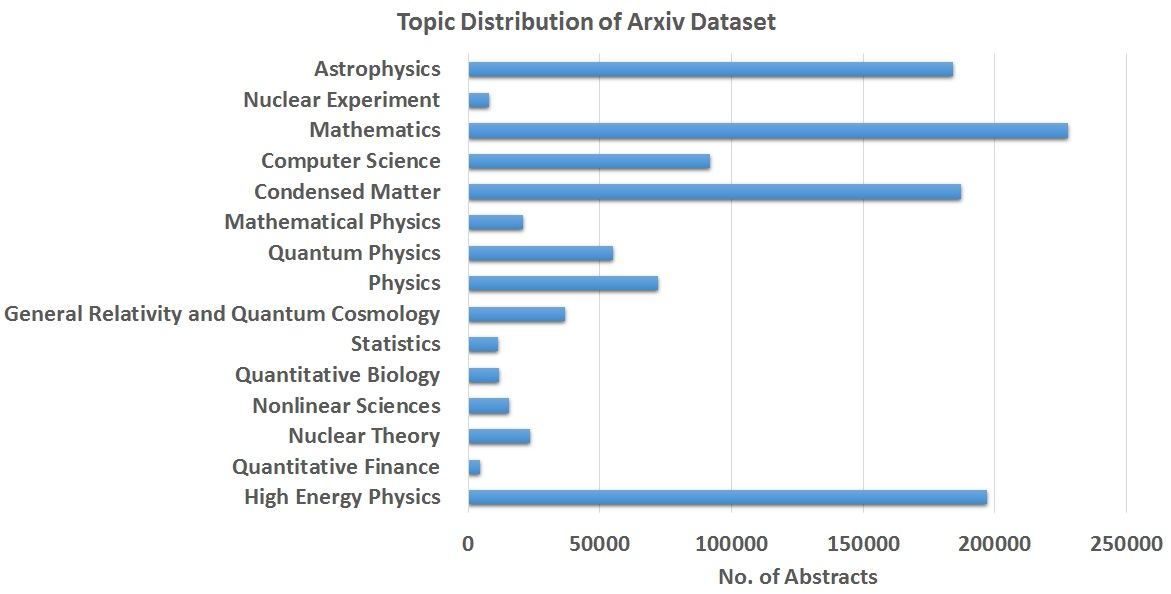
\includegraphics[width=9cm, height=6cm]{arxiv-topic-distribution.jpg}
\captionsetup{justification=centering}
  \caption{\small Frequency distribution of topics in the arxiv dataset.}
  \label{fig:arxiv-topics}
\end{figure}


\subsection{Evaluating Ranked Keyword Extraction}
We evaluate \textit{Key2Vec} by comparing it with the state-of-the-art systems, on two datasets: \textit{Inspec} dataset of ACM abstracts \cite{hulth2003improved}, representing short documents, and \textit{SemEval 2010} Task 5 dataset \cite{kim2010semeval}, representing longer documents. We don't implement any existing system for comparison, as we have found from our experience that it is often hard to get the best results by replicating other systems when the original implementation is not present. We directly take the best results for the benchmark datasets as reported in the literature and evaluate our system using the same metrics. In this section, we explain the evaluation metrics used, and present statistics and results for each of the benchmark datasets. Both the datasets are publicly available\footnote{https://github.com/snkim/AutomaticKeyphraseExtraction}. The datasets have training, development and testing data. We only use the test data for all our evaluations as used by all the other systems. Some general statistics for test data provided in both the corpus is presented in Table \ref{general-stats}.

\begin{table}[htbp]
\centering
\footnotesize
\caption{General Statistics for Inspec and SemEval 2010 benchmark datasets.}
\label{general-stats}
\begin{tabular}{|c|c|c|}
\hline
\textit{\textbf{Corpus Statistics}} & \textbf{Inspec} & \textbf{SemEval 2010} \\ \hline
\textbf{Type} & Abstract & Full Article \\ \hline
\textbf{No. of Documents} & 500 & 100 \\ \hline
\textbf{Avg No. of Unigram Tokens \cite{bougouin2013topicrank}} & 136.3 & 5179.6 \\ \hline
\textbf{Total No. of Annotated Keywords} &  & 3003 \\ \hline
\textbf{Avg No. of Annotated Keywords} &  & 30.03 \\ \hline
\textbf{Total No. of Candidates for Key2Vec} &  6100 & 47159 \\ \hline
\textbf{Avg No. of Candidates for Key2Vec} & 12.2 & 471.59 \\ \hline
\textbf{Total No. of Matches} & 3562 & 958 \\ \hline
\textbf{Accuracy} & 72.50\% & 31.90\% \\ \hline 
\end{tabular}
\end{table}


\subsubsection{Evaluation Metrics}
The ranked keywords are evaluated using exact match evaluation metric as used in SemEval 2010 Task 5 \cite{kim2010semeval}. We match the keywords in the annotated documents in the benchmark datasets with those generated by \textit{Key2Vec}, and calculate micro-averaged precision, recall and F-score ($\beta= 1$) as given in equations \ref{precision}, \ref{recall} and \ref{f1}, respectively. In the evaluation, we check the performance over the top 5, 10 and 15 candidates returned by \textit{Key2Vec}. While comparing the performance of \textit{Key2Vec} with other systems for the Inspec dataset, we only use F1@10 as the data for other measures are not available. In case of SemEval 2010 dataset, we directly compare our system's performance with the best system in the competition. Next, we present the evaluation results for both the benchmark datasets.

\begin{equation}
precision = \frac{correctly \ matched \ keywords}{total \ no. \ of \ extracted \ keywords}
\label{precision}
\end{equation}

\begin{equation}
recall = \frac{correctly \ matched \ keywords}{total \ no. \ of \ assigned \ keywords}
\label{recall}
\end{equation}

\begin{equation}
F1 = \frac{2\times precision\times recall}{precision + recall}
\label{f1}
\end{equation}



\subsubsection{Inspec \label{inspec}}
The Inspec dataset \cite{hulth2003improved} is composed of 2000 abstracts of scientific articles divided into sets of 1000, 500, and 500, as training, validation and test datasets respectively. Each document has two lists of keywords assigned by humans - \textit{controlled}, which are assigned by the authors, and \textit{uncontrolled}, which are freely assigned by the
readers. The controlled keywords are mostly abstractive, whereas the uncontrolled ones are mostly extractive \cite{wang2015using}. 

\begin{table}[htbp]
\centering
\footnotesize
\caption{My caption}
\tabcolsep=0.10cm
\scalebox{1.0}{
\begin{tabular}{|c|c|c|c|c|}
\hline
\textit{\textbf{\begin{tabular}[c]{@{}c@{}}Inspec\\ Uncontrolled\end{tabular}}} & \textbf{\begin{tabular}[c]{@{}c@{}}Key2Vec\\ (actual match)\end{tabular}} & \textbf{\begin{tabular}[c]{@{}c@{}}Some Algorithm\end{tabular}} & \multicolumn{1}{l|}{\textbf{SGRank}} & \textbf{TFIDF} \\ \hline
\textbf{Avg Precision@5} &  &  & NA &  \\ \hline
\textbf{Avg Recall@5} &  &  & NA &  \\ \hline
\textbf{Avg F1@5} &  &  & 29.16\% &  \\ \hline
\textbf{Avg Precision@10} &  &  & NA &  \\ \hline
\textbf{Avg Recall@10} &  &  & NA &  \\ \hline
\textbf{Avg F1@10} &  &  & 33.95\% &  \\ \hline
\textbf{Avg Precision@15} &  &  & NA &  \\ \hline
\textbf{Avg Recall@15} &  &  & NA &  \\ \hline
\textbf{Avg F1@15} &  &  & 33.66\% &  \\ \hline
\end{tabular}}
\label{my-label}
\end{table}

\begin{table}[htbp]
\centering
\footnotesize
\caption{My caption}
\tabcolsep=0.10cm
\scalebox{1.0}{
\begin{tabular}{|c|c|c|c|c|}
\hline
\textit{\textbf{\begin{tabular}[c]{@{}c@{}}Inspec\\ Controlled + \\ Uncontrolled\end{tabular}}} & \textbf{\begin{tabular}[c]{@{}c@{}}Key2Vec\\ (actual match)\end{tabular}} & \textbf{\begin{tabular}[c]{@{}c@{}}Some Algorithm\end{tabular}} & \multicolumn{1}{l|}{\textbf{SGRank}} & \textbf{TFIDF} \\ \hline
\textbf{Avg Precision@5} &  &  &  &  \\ \hline
\textbf{Avg Recall@5} &  &  &  &  \\ \hline
\textbf{Avg F1@5} &  &  &  &  \\ \hline
\textbf{Avg Precision@10} &  &  &  &  \\ \hline
\textbf{Avg Recall@10} &  &  &  &  \\ \hline
\textbf{Avg F1@10} &  &  &  &  \\ \hline
\textbf{Avg Precision@15} &  &  &  &  \\ \hline
\textbf{Avg Recall@15} &  &  &  &  \\ \hline
\textbf{Avg F1@15} &  &  &  &  \\ \hline
\end{tabular}}
\label{my-label}
\end{table}
\subsubsection{SemEval 2010 \label{semeval}}

The Semeval dataset was used in the Semeval 2010
keyphrase extraction shared task (Kim et al.,
2010). To the best of our knowledge this shared
task is the largest recent comparison of keyphrase
extraction algorithms and an algorithm’s
performance on this dataset is a relatively good
indication of where it stands compared to others in
the field. The Semeval dataset consists of 284 full
length ACM articles divided into a test set of size
100, training set of size 144 and trial set of size 40
which we used as the development set for
parameter tuning. Each article has two sets of
human assigned keyphrases: the author-assigned
and reader-assigned ones. The gold standard used
in our experiments is the combined set of author
and reader assigned keyphrases which is the same
as was done in the Semeval shared task. The table
below provides a statistical overview of this
dataset’s documents.

\textit{Table showing Semeval 2010 dataset statistics}

\begin{table}[htbp]
\footnotesize
\centering
\caption{My caption}
\begin{tabular}{|c|c|c|c|c|}
\hline
\textbf{\begin{tabular}[c]{@{}c@{}}SemEval 2010 \\ Combined\end{tabular}} & \textbf{\begin{tabular}[c]{@{}c@{}}Key2Vec \\ (actual match)\end{tabular}} & \textbf{\begin{tabular}[c]{@{}c@{}}Some Algorithm\end{tabular}} & \textbf{HUMB} & \textbf{TFIDF} \\ \hline
\textbf{Avg Precision@5} & 41\% &  & 39.00\% &  \\ \hline
\textbf{Avg Recall@5} & 14.37\% &  & 13.30\% &  \\ \hline
\textbf{Avg F1@5} & 21.28\% &  & 19.80\% &  \\ \hline
\textbf{Avg Precision@10} & 35.29\% &  & 32.00\% &  \\ \hline
\textbf{Avg Recall@10} & 24.67\% &  & 21.80\% &  \\ \hline
\textbf{Avg F1@10} & 29.04\% &  & 26.00\% &  \\ \hline
\textbf{Avg Precision@15} & 34.39\% &  & 27.20\% &  \\ \hline
\textbf{Avg Recall@15} & 32.48\% &  & 27.80\% &  \\ \hline
\textbf{Avg F1@15} & 33.41\% &  & 27.50\% &  \\ \hline
\end{tabular}
\label{my-label}
\end{table}


\begin{table}[htbp]
\centering
\footnotesize
\caption{My caption}
\begin{tabular}{|c|c|c|c|c|}
\hline
\textbf{\begin{tabular}[c]{@{}c@{}}SemEval 2010 \\ Combined\end{tabular}} & \textbf{\begin{tabular}[c]{@{}c@{}}Key2Vec \\ (actual match)\end{tabular}} & \textbf{\begin{tabular}[c]{@{}c@{}}Some Algorithm\end{tabular}} & \textbf{HUMB} & \textbf{TFIDF} \\ \hline
\textbf{Avg Precision@5} & 38.20\% &  & 30.40\% &  \\ \hline
\textbf{Avg Recall@5} & 15.97\% &  & 12.60\% &  \\ \hline
\textbf{Avg F1@5} & 22.52\% &  & 17.80\% &  \\ \hline
\textbf{Avg Precision@10} & 31.68\% &  & 24.80\% &  \\ \hline
\textbf{Avg Recall@10} & 26.25\% &  & 20.60\% &  \\ \hline
\textbf{Avg F1@10} & 28.71\% &  & 22.50\% &  \\ \hline
\textbf{Avg Precision@15} & 34.92\% &  & 12.10\% &  \\ \hline
\textbf{Avg Recall@15} & 34.39\% &  & 47.00\% &  \\ \hline
\textbf{Avg F1@15} & 34.65\% &  & 19.30\% &  \\ \hline
\end{tabular}
\label{my-label}
\end{table}

We have compared our algorithm with KPMiner
and TextRank using only the 100 documents
in the test set. The following diagram shows the
average precision and recall achieved by each
algorithm. As was done in the Semeval task,
comparisons are done between once stemmed
human assigned keyphrases and ranked candidates
returned by each algorithm.

\begin{table}[htbp]
\footnotesize
\centering
\caption{My caption}
\tabcolsep=0.11cm
\scalebox{0.9}{\begin{tabular}{|c|c|c|c|c|c|}
\hline
\textbf{\begin{tabular}[c]{@{}c@{}}SemEval 2010 \\ Combined \\ (Raw Text)\end{tabular}} & \textbf{title} & \textbf{\begin{tabular}[c]{@{}c@{}}title + \\ abstract\end{tabular}} & \textbf{\begin{tabular}[c]{@{}c@{}}title + \\ introduction\end{tabular}} & \textbf{\begin{tabular}[c]{@{}c@{}}title + \\ abstract + \\ introduction+ \\ conclusion\end{tabular}} & \textbf{full article} \\ \hline
\textbf{Avg Precision@5} & 41.40\% & 40.60\% & 41.20\% & 41\% & 41\% \\ \hline
\textbf{Avg Recall@5} & 14.56\% & 14.24\% & 14.48\% & 14.40\% & 14.37\% \\ \hline
\textbf{Avg F1@5} & 21.54\% & 21.09\% & 21.43\% & 21.32\% & 21.28\% \\ \hline
\textbf{Avg Precision@10} & 35.29\% & 35.09\% & 35.09\% & 34.99\% & 35.29\% \\ \hline
\textbf{Avg Recall@10} & 24.66\% & 24.51\% & 24.51\% & 24.45\% & 24.67\% \\ \hline
\textbf{Avg F1@10} & 29.04\% & 28.86\% & 28.86\% & 28.79\% & 29.04\% \\ \hline
\textbf{Avg Precision@15} & 34.40\% & 34.53\% & 34.68\% & 34.53\% & 34.39\% \\ \hline
\textbf{Avg Recall@15} & 32.45\% & 32.60\% & 32.75\% & 32.60\% & 32.48\% \\ \hline
\textbf{Avg F1@15} & 33.40\% & 33.54\% & 33.69\% & 33.54\% & 33.41\% \\ \hline
\end{tabular}}
\label{my-label}
\end{table}


%\begin{table*}[htbp]
%\footnotesize
%\centering
%\caption{My caption}
%\begin{tabular}{|c|c|c|c|c|c|}
%\hline
%\textbf{\begin{tabular}[c]{@{}c@{}}SemEval 2010 \\ Reader Assigned \\ (Raw Text)\end{tabular}} & \textbf{title} & \textbf{\begin{tabular}[c]{@{}c@{}}title + \\ abstract\end{tabular}} & \textbf{\begin{tabular}[c]{@{}c@{}}title + \\ introduction\end{tabular}} & \textbf{\begin{tabular}[c]{@{}c@{}}title + \\ abstract + \\ introduction+ \\ conclusion\end{tabular}} & \textbf{full article} \\ \hline
%\textbf{\begin{tabular}[c]{@{}c@{}}Avg \\ Precision@5\end{tabular}} & 38.60\% & 37.80\% & 38.40\% & 38.20\% & 38.20\% \\ \hline
%\textbf{\begin{tabular}[c]{@{}c@{}}Avg \\ Recall@5\end{tabular}} & 16.17\% & 15.82\% & 16.08\% & 16.00\% & 15.97\% \\ \hline
%\textbf{\begin{tabular}[c]{@{}c@{}}Avg \\ F1@5\end{tabular}} & 22.79\% & 22.31\% & 22.67\% & 22.56\% & 22.52\% \\ \hline
%\textbf{\begin{tabular}[c]{@{}c@{}}Avg \\ Precision@10\end{tabular}} & 31.69\% & 31.48\% & 31.48\% & 31.38\% & 31.68\% \\ \hline
%\textbf{\begin{tabular}[c]{@{}c@{}}Avg \\ Recall@10\end{tabular}} & 26.24\% & 26.07\% & 26.06\% & 25.99\% & 26.25\% \\ \hline
%\textbf{\begin{tabular}[c]{@{}c@{}}Avg \\ F1@10\end{tabular}} & 28.71\% & 28.52\% & 28.51\% & 28.43\% & 28.71\% \\ \hline
%\textbf{\begin{tabular}[c]{@{}c@{}}Avg \\ Precision@15\end{tabular}} & 34.89\% & 35.04\% & 35.24\% & 35.04\% & 34.92\% \\ \hline
%\textbf{\begin{tabular}[c]{@{}c@{}}Avg \\ Recall@15\end{tabular}} & 34.35\% & 34.51\% & 34.71\% & 34.51\% & 34.39\% \\ \hline
%\textbf{\begin{tabular}[c]{@{}c@{}}Avg \\ F1@15\end{tabular}} & 34.62\% & 34.77\% & 34.97\% & 34.77\% & 34.65\% \\ \hline
%\end{tabular}
%\label{my-label}
%\end{table*}


\begin{table}[htbp]
\footnotesize
\centering
\caption{My caption}
\tabcolsep=0.11cm
\scalebox{0.9}{
\begin{tabular}{|c|c|c|c|c|c|}
\hline
\textbf{\begin{tabular}[c]{@{}c@{}}SemEval 2010 \\ Combined \\ (Preprocessed)\end{tabular}} & \textbf{title} & \textbf{\begin{tabular}[c]{@{}c@{}}title + \\ abstract\end{tabular}} & \textbf{\begin{tabular}[c]{@{}c@{}}title + \\ introduction\end{tabular}} & \textbf{\begin{tabular}[c]{@{}c@{}}title + \\ abstract + \\ introduction+ \\ conclusion\end{tabular}} & \textbf{full article} \\ \hline
\textbf{Avg Precision@5} & 43.80\% & 43.80\% & 43.80\% & 44\% & 43.80\% \\ \hline
\textbf{Avg Recall@5} & 15.08\% & 15.08\% & 15.08\% & 15.18\% & 15.08\% \\ \hline
\textbf{Avg F1@5} & 22.44\% & 22.44\% & 22.44\% & 22.57\% & 22.44\% \\ \hline
\textbf{Avg Precision@10} & 37.39\% & 37.49\% & 37.19\% & 36.99\% & 37.19\% \\ \hline
\textbf{Avg Recall@10} & 25.86\% & 25.95\% & 25.76\% & 25.59\% & 25.77\% \\ \hline
\textbf{Avg F1@10} & 30.57\% & 30.67\% & 30.44\% & 30.25\% & 30.44\% \\ \hline
\textbf{Avg Precision@15} & 37.96\% & 37.61\% & 37.61\% & 37.69\% & 37.77\% \\ \hline
\textbf{Avg Recall@15} & 35.62\% & 35.34\% & 35.35\% & 35.37\% & 35.50\% \\ \hline
\textbf{Avg F1@15} & 36.75\% & 36.44\% & 36.44\% & 36.49\% & 36.60\% \\ \hline
\end{tabular}}
\label{my-label}
\end{table}


%\begin{table*}[htbp]
%\footnotesize
%\centering
%\caption{My caption}
%\begin{tabular}{|c|c|c|c|c|c|}
%\hline
%\textbf{\begin{tabular}[c]{@{}c@{}}SemEval 2010 \\ Reader Assigned\\ (Preprocessed)\end{tabular}} & \textbf{title} & \textbf{\begin{tabular}[c]{@{}c@{}}title + \\ abstract\end{tabular}} & \textbf{\begin{tabular}[c]{@{}c@{}}title + \\ introduction\end{tabular}} & \textbf{\begin{tabular}[c]{@{}c@{}}title + \\ abstract + \\ introduction+ \\ conclusion\end{tabular}} & \textbf{full article} \\ \hline
%\textbf{Avg Precision@5} & 39.80\% & 39.80\% & 39.80\% & 40\% & 39.80\% \\ \hline
%\textbf{Avg Recall@5} & 16.57\% & 16.57\% & 16.57\% & 16.68\% & 16.57\% \\ \hline
%\textbf{Avg F1@5} & 23.39\% & 23.39\% & 23.39\% & 23.54\% & 23.39\% \\ \hline
%\textbf{Avg Precision@10} & 33.62\% & 33.72\% & 33.62\% & 33.32\% & 33.42\% \\ \hline
%\textbf{\begin{tabular}[c]{@{}c@{}}Avg \\ Recall@10\end{tabular}} & 27.73\% & 27.84\% & 27.78\% & 27.45\% & 27.60\% \\ \hline
%\textbf{\begin{tabular}[c]{@{}c@{}}Avg \\ F1@10\end{tabular}} & 30.40\% & 30.50\% & 30.42\% & 30.10\% & 30.23\% \\ \hline
%\textbf{\begin{tabular}[c]{@{}c@{}}Avg \\ Precision@15\end{tabular}} & 38.51\% & 38.19\% & 38.22\% & 38.25\% & 38.33\% \\ \hline
%\textbf{\begin{tabular}[c]{@{}c@{}}Avg \\ Recall@15\end{tabular}} & 37.82\% & 37.52\% & 37.56\% & 37.55\% & 37.67\% \\ \hline
%\textbf{\begin{tabular}[c]{@{}c@{}}Avg \\ F1@15\end{tabular}} & 38.16\% & 37.85\% & 37.89\% & 37.90\% & 38.00\% \\ \hline
%\end{tabular}
%\label{my-label}
%\end{table*}


%\begin{table}
%\small
%\begin{tabular}{cc|c|c|c|c|c|c|c|c|}
%\cline{3-10}
%\textbf{\shortstack{\underline{Phrase-Sentence} \\ \underline{Similarity}}}&  & \multicolumn{8}{ c| }{\textbf{Dimensions}} \\ \cline{3-10}
%\textbf{Models}& & \textbf{10} & \textbf{25} & \textbf{50} & \textbf{75} & \textbf{100} & \textbf{500} & \textbf{1000} & \textbf{1500}\\ \cline{1-10}
%word2vec skipgram &  &  &  &  &  &  &  &  \\ \hline
%\end{tabular}
%\end{table}


\section{Discussion \label{discussion}}

\section{Future Work and Conclusion \label{conclusion}}


% needed in second column of first page if using \IEEEpubid
%\IEEEpubidadjcol

% An example of a floating figure using the graphicx package.
% Note that \label must occur AFTER (or within) \caption.
% For figures, \caption should occur after the \includegraphics.
% Note that IEEEtran v1.7 and later has special internal code that
% is designed to preserve the operation of \label within \caption
% even when the captionsoff option is in effect. However, because
% of issues like this, it may be the safest practice to put all your
% \label just after \caption rather than within \caption{}.
%
% Reminder: the "draftcls" or "draftclsnofoot", not "draft", class
% option should be used if it is desired that the figures are to be
% displayed while in draft mode.
%
%\begin{figure}[!t]
%\centering
%\includegraphics[width=2.5in]{myfigure}
% where an .eps filename suffix will be assumed under latex, 
% and a .pdf suffix will be assumed for pdflatex; or what has been declared
% via \DeclareGraphicsExtensions.
%\caption{Simulation Results}
%\label{fig_sim}
%\end{figure}

% Note that IEEE typically puts floats only at the top, even when this
% results in a large percentage of a column being occupied by floats.


% An example of a double column floating figure using two subfigures.
% (The subfig.sty package must be loaded for this to work.)
% The subfigure \label commands are set within each subfloat command, the
% \label for the overall figure must come after \caption.
% \hfil must be used as a separator to get equal spacing.
% The subfigure.sty package works much the same way, except \subfigure is
% used instead of \subfloat.
%
%\begin{figure*}[!t]
%\centerline{\subfloat[Case I]\includegraphics[width=2.5in]{subfigcase1}%
%\label{fig_first_case}}
%\hfil
%\subfloat[Case II]{\includegraphics[width=2.5in]{subfigcase2}%
%\label{fig_second_case}}}
%\caption{Simulation results}
%\label{fig_sim}
%\end{figure*}
%
% Note that often IEEE papers with subfigures do not employ subfigure
% captions (using the optional argument to \subfloat), but instead will
% reference/describe all of them (a), (b), etc., within the main caption.


% An example of a floating table. Note that, for IEEE style tables, the 
% \caption command should come BEFORE the table. Table text will default to
% \footnotesize as IEEE normally uses this smaller font for tables.
% The \label must come after \caption as always.
%
%\begin{table}[!t]
%% increase table row spacing, adjust to taste
%\renewcommand{\arraystretch}{1.3}
% if using array.sty, it might be a good idea to tweak the value of
% \extrarowheight as needed to properly center the text within the cells
%\caption{An Example of a Table}
%\label{table_example}
%\centering
%% Some packages, such as MDW tools, offer better commands for making tables
%% than the plain LaTeX2e tabular which is used here.
%\begin{tabular}{|c||c|}
%\hline
%One & Two\\
%\hline
%Three & Four\\
%\hline
%\end{tabular}
%\end{table}


% Note that IEEE does not put floats in the very first column - or typically
% anywhere on the first page for that matter. Also, in-text middle ("here")
% positioning is not used. Most IEEE journals use top floats exclusively.
% Note that, LaTeX2e, unlike IEEE journals, places footnotes above bottom
% floats. This can be corrected via the \fnbelowfloat command of the
% stfloats package.








% if have a single appendix:
%\appendix[Proof of the Zonklar Equations]
% or
%\appendix  % for no appendix heading
% do not use \section anymore after \appendix, only \section*
% is possibly needed

% use appendices with more than one appendix
% then use \section to start each appendix
% you must declare a \section before using any
% \subsection or using \label (\appendices by itself
% starts a section numbered zero.)
%







% Can use something like this to put references on a page
% by themselves when using endfloat and the captionsoff option.
\ifCLASSOPTIONcaptionsoff
  \newpage
\fi



% trigger a \newpage just before the given reference
% number - used to balance the columns on the last page
% adjust value as needed - may need to be readjusted if
% the document is modified later
%\IEEEtriggeratref{8}
% The "triggered" command can be changed if desired:
%\IEEEtriggercmd{\enlargethispage{-5in}}

% references section

% can use a bibliography generated by BibTeX as a .bbl file
% BibTeX documentation can be easily obtained at:
% http://www.ctan.org/tex-archive/biblio/bibtex/contrib/doc/
% The IEEEtran BibTeX style support page is at:
% http://www.michaelshell.org/tex/ieeetran/bibtex/
%\bibliographystyle{IEEEtran}
% argument is your BibTeX string definitions and bibliography database(s)
%\bibliography{IEEEabrv,../bib/paper}
%
% <OR> manually copy in the resultant .bbl file
% set second argument of \begin to the number of references
% (used to reserve space for the reference number labels box)
%\begin{thebibliography}{1}
\bibliographystyle{IEEEtran}
\bibliography{cikm}

%\end{thebibliography}

% biography section
% 
% If you have an EPS/PDF photo (graphicx package needed) extra braces are
% needed around the contents of the optional argument to biography to prevent
% the LaTeX parser from getting confused when it sees the complicated
% \includegraphics command within an optional argument. (You could create
% your own custom macro containing the \includegraphics command to make things
% simpler here.)
%\begin{biography}[{\includegraphics[width=1in,height=1.25in,clip,keepaspectratio]{mshell}}]{Michael Shell}
% or if you just want to reserve a space for a photo:

\begin{IEEEbiography}[{\includegraphics[width=1in,height=1.25in,clip,keepaspectratio]{picture}}]{John Doe}
\blindtext
\end{IEEEbiography}

% You can push biographies down or up by placing
% a \vfill before or after them. The appropriate
% use of \vfill depends on what kind of text is
% on the last page and whether or not the columns
% are being equalized.

%\vfill

% Can be used to pull up biographies so that the bottom of the last one
% is flush with the other column.
%\enlargethispage{-5in}




% that's all folks
\end{document}


